\documentclass{my_paper}
\usepackage{ctex}
\usepackage[textwidth=444bp,vmargin=2.5cm]{geometry}%设置页边距
\usepackage{array} %主要是增加列样式选项
\usepackage[dvipsnames]{xcolor}%颜色宏包
\usepackage{graphicx}%图片宏包
\usepackage{amsmath}%公式宏包
\usepackage{amsthm}
\usepackage[T1]{fontenc}    
\usepackage{newtxtext, newtxmath}  %两种使用Times New Roman 字体的方法
\usepackage[english]{babel}
\newcommand{\R}{\mathbb{R}}
\newtheorem{theorem}{Theorem}
\newtheorem{corollary}{Corollary}[theorem]
\newtheorem{lemma}[theorem]{Lemma}

\begin{document}
%----------- 中文摘要 ----------
\newpage

\begin{center}
\lunwenbiaoti

\vspace{2ex}
\zhaiyao
\end{center}

开头段:需要充分概括论文内容,一般两到三句话即可,长度控制在三至五行。

问题一中,解决了什么问题;应用了什么方法;得到了什么结果。

问题二中,解决了什么问题;应用了什么方法;得到了什么结果。

问题三中,解决了什么问题;应用了什么方法;得到了什么结果。

结尾段:可以总结下全文,也可以介绍下你的论文的亮点,也可以对类似的问题进行适当的推广。

\begin{guanjianci}
关键词一 \quad 关键词二 \quad 关键词三
\end{guanjianci}

%----------- 正文 ----------
%----------- 一、问题重述 ----------
\newpage
\section{一、问题重述}
在无人机集群飞行的过程中,采用了纯方位无源定位的方法来保持无人机集群的编队队形。纯方位无源定位方法如下:编队中选择几架无人机发射信号,其余无人机接受信号,约定该无人机与任意两家发射方无人机连线之间的夹角信息是接收方无人机接收到的信息。
所有无人机都有各自的固定编号且相对位置保持不变。同时为了避免外界的干扰,无人机飞行过程中应尽量避免信号的收发。为了帮助无人机定位并且调整位置,我们需要针对以下两个情形建立数学模型完成以下任务:\\
情景1: 10架无人机组成圆形编队,1架位于圆心,另外9架均匀分布于圆周上。  \\
1. 编号已知且位置无偏差的圆心无人机和另外2架无人机向其他无人机发送信号,建立接收信号无人机定位模型。 \\
2. 位置已知、编号为FY00和FY01的无人机发射信号,寻找能够满足有效无人机定位需要的额外发送编号未知无人机最少数量。 \\
3. 当初始时刻无人机位置略有偏差时,在至多只能选择圆心无人机以及另外3架无人机发送信号的限制下,寻找调整到理想位置的策略并以表1的数据进行模拟。 \\
情形2: 无人机集群编队队形为锥形编队队形,线上相邻两架无人机间距相等。 \\
1. 通过建立的模型得到相应的无人机位置调整策略

%----------- 二、问题分析 ----------
\section{二、问题分析}
\subsection{问题一的分析}
问题一分为三个小问题。第一小问要求根据三架编号已知且位置没有偏差的信号机来给出任何一架无人机的定位系统。在第一问下,由于所有角度信息已知,一个方面,如果考虑信号机本身的位置问题,分类情况会变得复杂,因此我们将信号机中两架外机和内机形成的夹角作为变量纳入模型考虑,利用接收机和信号机之间固定夹角形成的圆弧,来对接收机进行定位,因此得到一个普适的定位模型。另一方面,对于不同的接收机位置,它和相同信号机之间的夹角所提供的信息是不同的,因此我们引入夹角的正负型。为了防止过多的分类情况导致模型的适用性降低,我们对正负夹角的所有组合都进行计算,并选择出结果正确的一组。\\

第二小问当中隐去了一台无人机的编号信息,\\

第三小问需要我们更进一步,对无人机的位置偏差进行调整,让它们最后均匀分布在某个圆周上,同时不保证信号机自身位置的正确。为了进一步增加我们的固有信息,我们利用FY00和FY01的位置信息作为正确的位置信息,并通过FY01,FY04,FY07在理想情况下构成的等边三角形,让FY04和FY07相互作为信号机进行位置调整。我们证明了在这种情况下FY04和FY07在这种调整方案下能够以较快的速度向正确位置收敛,并最终得到四个正确的相对位置信息。利用这四架无人机中的三架,就可以在下一步完成所有无人机的位置调整。
\subsection{问题二的分析}
这是你的内容这是你的内容这是你的内容这是你的内容这是你的内容这是你的内容这是你的内容
%----------- 三、模型假设 ----------
\section{三、模型假设}
为了构建更为精确的数学模型,本文根据实际情况作出以下的假设或条件约束:

假设一:在不进行位置调整时,无人机之间的相对位置在行进中保持不变。

假设二:所有的无人机在同一高度飞行

假设三:无人机的位置偏差在可接受的范围内。

假设四:不考虑无人机在行进过程中产生的意外情况。
%----------- 四、符号说明 ----------
\section{四、符号说明}
%使用三线表格最好~
\begin{table}[h]%htbp表示的意思是latex会尽量满足排在前面的浮动格式,就是h-t-b-p这个顺序,让排版的效果尽量好。
    \centering
    \begin{tabular}{p{2.0cm}<{\centering}p{9.0cm}<{\centering}p{2.0cm}<{\centering}}
 %指定单元格宽度, 并且水平居中。
    \hline
    符号 & 说明 & 单位 \\ %换行 
    \hline
    $\int$ & 积分符号 &  \\ %把你的符号写在这
    $W_0$ & 区分高峰和低峰的一个临界值 &  \\ %把你的符号写在这
    $M_t$ &  简单移动平均项 &  \\ %把你的符号写在这
    \hline
    \end{tabular}
\end{table}
本部分是对模型中使用的重要变量进行说明,一般排版时要放到一张表格中。

注意:第一:不需要把所有变量都放到这个表里面,模型中用到的临时变量可以不放。第二:下文中首次出现这些变量时也要进行解释,不然会降低文章的可读性。

%----------- 五、模型的建立与求解 ----------
\section{五、模型的建立与求解}

(注意:这个部分里面的标题可根据你的论文内容进行调整,我这里给的是一个通用的模版)

\subsection{第一问:无人机定位系统的建立}
\subsubsection{模型准备}
1)信号机的位置关系:

由于在理想情况下,九架外机均匀分布在圆周上,且飞行高度相同,因此对于不同的信号机的位置关系,只需要考虑两架外机之间的相对位置作为情况划分。因此,不妨假设其中一架外机为FY01,则只需要考虑以下四种位置关系:


\subsubsection{模型求解}

\subsection{第二问模型的建立与求解}

\subsection{第三问模型的建立与求解}
    注意到理想情况下FY01,FY04,FY07构成一个等边三角形,FY00是它的中心。第一步我们将固定FY00和FY01,
    通过反复调整FY04和FY07,使得FY01,FY04,FY07构成以FY00为中心的等边三角形。下面的定理保证了这样
    调整进行得很快。
\begin{theorem}[等边三角形定理]
\label{dbsjx} 
    设 $O=(0,0)$, $C=(1,0)$,   
    $A^{(0)}=(1+\Delta,-\frac{2\pi}3-\delta)\in \R^{\geq 0}\times S^1$. 用如下递归的方式构造点列
    $\{B^{(i)}\}_{i\geq 1}$, $\{A^{(i)}\}_{i\geq 1}$: 
    $B^{(i)}=(r_B^{(i)},\theta_B^{(i)})$, $\theta_{B}^{(i)}\in (\frac \pi 2,\pi)$ 是
    第二象限中满足 $\angle CB^{(i)}O=\angle OB^{(i)}A^{(i-1)}=\frac\pi6$ 的点, 
    $A^{(i)}=(r_A^{(i)},-\theta_A^{(i)})$, $\theta_{A}^{(i)}\in (\frac \pi 2,\pi)$ 是
    第三象限中满足 $\angle CA^{(i)}O=\angle OA^{(i)}B^{(i)}=\frac\pi6$ 的点(接下来构造 $B^{(i+1)}$, $A^{(i+1)})$. 
    则 
    \begin{equation}
    \begin{aligned}
        r_A^{(i)}=1+o((|\Delta|+|\delta|)^{(i)}),\quad r_B^{(i)}=1+o((|\Delta|+|\delta|)^{(i-1)}),
        \\
        \theta_A^{(i)}=\frac{2\pi}{3}+o((|\Delta|+|\delta|)^{(i)}),\quad \theta_B^{(i)}=\frac{2\pi}{3}+o((|\Delta|+|\delta|)^{(i-1)}).
    \end{aligned}
    \label{1}
    \end{equation}
    利用有限维 Banach 空间的范数等价性, 有序列 $A^{(i)}$, $B^{(i)}$ 分别依2-范数超线性收敛到
    (converge superlinearly under Euclidean norm to) $(1,\frac{-2\pi}3)$, $(1,\frac{2\pi}3)$.
\end{theorem} 

\begin{figure}[h]
    \centering
    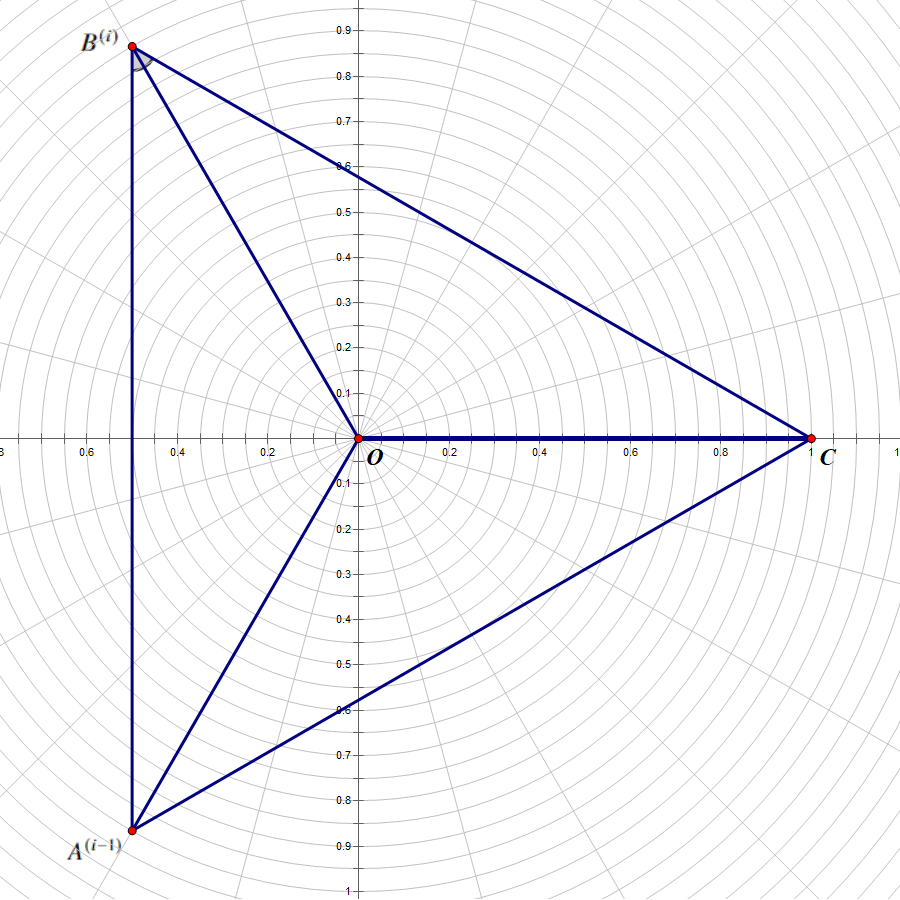
\includegraphics[width=0.5\textwidth]{sketch1}
    \caption{从 $A^{(i-1)}$ 构造 $B^{(i)}$ 的过程} 
\end{figure}

\begin{proof}
    不妨设 $r_A^{(i-1)}=1+\Delta_A^{(i-1)}$, $\theta_A^{(i-1)}=\frac{2\pi}{3}+\delta_A^{(i-1)}$. 根据几何关系,有 
    $$
    r_A^{i-1}\sin(\theta_B^{(i)}+\theta_A^{(i-1)}-\frac{7\pi}{6})=\sin(\frac{5\pi}{6}-\theta_{B}^{(i)})=\frac12 r_B^{(i)}.
    $$
    做 Taylor 展开,忽略一阶小就有
    $$
        \theta_{B}^{(i)}= \frac{2\pi}3-\frac{1}{2} \delta_A^{(i-1)}-\frac{\sqrt 3}6 \Delta_A^{(i-1)}+o(|\Delta_A^{(i-1)}|+|\delta_A^{(i-1)}|)
        ,\quad r_{B}^{(i)} = 1 +\frac{\sqrt3}{2} \delta_A^{(i-1)}+\frac12 \Delta_A^{(i-1)}+o((|\Delta_A^{(i-1)}|+|\delta_A^{(i-1)}|).
    $$
    利用旋转对称性,可得
    \begin{equation}
    \begin{aligned}
        \theta_{A}^{(i)}= \frac{2\pi}3-\frac{1}{2} (-\frac{1}{2} \delta_A^{(i-1)}-\frac{\sqrt 3}6 \Delta_A^{(i-1)})
        -\frac{\sqrt 3}6 (\frac{\sqrt3}{2} \delta_A^{(i-1)}+\frac12 \Delta_A^{(i-1)}) +o(|\Delta_A^{(i-1)}|+|\delta_A^{(i-1)}|)
        \\=o(|\Delta_A^{(i-1)}|+|\delta_A^{(i-1)}|).&
    \end{aligned}
    \label{2}
    \end{equation}
    同理 $r_{A}^{(i)}=o(|\Delta_A^{(i-1)}|+|\delta_A^{(i-1)}|).$ 利用数学归纳法可得结果. 
\end{proof}

\subsection{问题二模型的建立与求解}



%----------- 六、模型的分析与检验 ----------
\section{六、模型的分析与检验}

模型的分析与检验的内容也可以放到模型的建立与求解部分,这里我们单独抽出来进行讲解,因为这部分往往是论文的加分项,很多优秀论文也会单独抽出一节来对这个内容进行讨论。

模型的分析 :在建模比赛中模型分析主要有两种,一个是灵敏度(性)分析,另一个是误差分析。灵敏度分析是研究与分析一个系统(或模型)的状态或输出变化对系统参数或周围条件变化的敏感程度的方法。其通用的步骤是:控制其他参数不变的情况下,改变模型中某个重要参数的值,然后观察模型的结果的变化情况。误差分析是指分析模型中的误差来源,或者估算模型中存在的误差,一般用于预测问题或者数值计算类问题。

模型的检验:模型检验可以分为两种,一种是使用模型之前应该进行的检验,例如层次分析法中一致性检验,灰色预测中的准指数规律的检验,这部分内容应该放在模型的建立部分;另一种是使用了模型后对模型的结果进行检验,数模中最常见的是稳定性检验,实际上这里的稳定性检验和前面的灵敏度分析非常类似。

\section{七、模型的评价、改进与推广}
注:本部分的标题需要根据你的内容进行调整,例如:如果你没有写模型推广的话,就直接把标题写成模型的评价与改进。很多论文也把这部分的内容直接统称为“模型评价”部分,也是可以的。

\subsection{模型的优点}
优缺点是必须要写的内容,改进和推广是可选的,但还是建议大家写,实力比较强的建模者可以在这一块充分发挥,这部分对于整个论文的作用在于画龙点睛。
\subsection{模型的缺点}
缺点写的个数要比优点少
\subsection{模型的改进}
主要是针对模型中缺点有哪些可以改进的地方\cite{risken1996fokker};
\subsection{模型的推广}
将原题的要求进行扩展\cite{rossler1979equation},进一步讨论模型的实用性和可行性\cite{mckean1970nagumo}。

%----------- 参考文献 ----------
\bibliographystyle{unsrt} %规定了参考文献的格式
\begin{center}
\bibliography{reference} %调出LaTeX生成参考文献列表
\end{center}
\textcolor{red}{(所有引用他人或公开资料(包括网上资料)的成果必须按照科技论文的规范列出参考文献,并在正文引用处予以标注。}

\textcolor{red}{常见的三种参考文献的表达方式(标准不唯一):
书籍的表述方式为: [编号] 作者,书名,出版地:出版社,出版年月。
期刊杂志论文的表述方式为: [编号] 作者,论文名,杂志名,卷期号:起止页码,出版年。
网上资源(例如数据库、政府报告)的表述方式为: [编号] 作者,资源标题,网址,访问时间。)}
%----------- 附录 ----------
\newpage
\section{附录}

\begin{table}[htbp]
    \centering
    \begin{tabular}{|p{14.0cm}|}
 %指定单元格宽度, 并且水平居中。
    \hline
    \textbf{附录1} \\ %换行 
    \hline
    介绍:支撑材料的文件列表  \\ 
    \\
    \\
    \\
    \hline
    \end{tabular}
\end{table}

\begin{table}[htbp]
    \centering
    \begin{tabular}{|p{14.0cm}|}
 %指定单元格宽度, 并且水平居中。
    \hline
    \textbf{附录2} \\ %换行 
    \hline
    介绍:该代码是某某语言编写的,作用是什么   \\ 
    \\
    \\
    \\
    \hline
    \end{tabular}
\end{table}

除了支撑材料的文件列表和源程序代码外,附录中还可以包括下面内容:
\begin{itemize}
\item 某一问题的详细证明或求解过程;
\item 自己在网上找到的数据;
\item 比较大的流程图;
\item 较繁杂的图表或计算结果
\end{itemize}

\end{document}